\begin{figure}
    \centering
    %\tikzstyle{block} = [rectangle, rounded corners, text=black, text centered, draw=black, minimum height=.3in]
    %\tikzstyle{block} = [rectangle, rounded corners, text=black, text centered, draw=black,font=\scriptsize, minimum height=.35in, minimum width=.65in]
    \tikzstyle{block} = [rectangle, rounded corners, text=black, text centered, draw=black,font=\scriptsize, minimum width=.65in, minimum height=.2in]
    \tikzstyle{line} = [-latex,draw=black,line width=.4]
    \tikzstyle{line2} = [latex-latex,draw=black,line width=.4, dashed]
    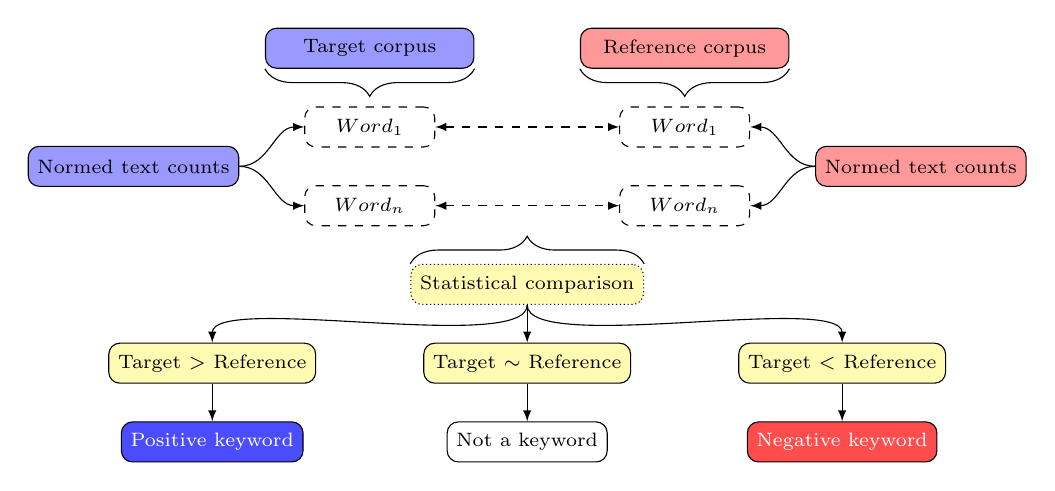
\begin{tikzpicture}
        %\node[block,fill=black!50,text=white] (kwanalysis) at (10,10) {Keyword analysis};
        \node[block,fill=blue!40,text=black,text width=.95in] (target) at (8,9) {Target corpus};
        \node[block,fill=red!40,text=black,text width=.95in] (reference) at (12,9) {Reference corpus};
        \node[block,fill=blue!40,text=black] (textcounts1) at (5,7.5) {Normed text counts};
        \node[block,fill=red!40,text=black] (textcounts2) at (15,7.5) {Normed text counts};
        \node[block,text=black,text width=.55in, dashed] (word1left) at (8,8) {$Word_1$};
        \node[block,text=black,text width=.55in, dashed] (word1right) at (12,8) {$Word_1$};
        \node[block,text=black,text width=.55in, dashed] (word2left) at (8,7) {$Word_n$};
        \node[block,text=black,text width=.55in, dashed] (word2right) at (12,7) {$Word_n$};
        \node[block,fill=yellow!30,text=black,densely dotted] (comparison) at (10,6) {Statistical comparison};
        \node[block,fill=yellow!30,text=black] (greater) at (6,5) {Target $>$ Reference};
        %\node[block,fill=yellow!30,text=black] (similar) at (10,5) {Target $\simeq$ Reference};
        %\node[block,fill=yellow!30,text=black] (similar) at (10,5) {Target $\approx$ Reference};
        \node[block,fill=yellow!30,text=black] (similar) at (10,5) {Target $\sim$ Reference};
        \node[block,fill=yellow!30,text=black] (lesser) at (14,5) {Target $<$ Reference};
        \node[block,fill=blue!70,text=white] (poskw) at (6,4) {Positive keyword};
        \node[block,text=black] (notkw) at (10,4) {Not a keyword};
        \node[block,fill=red!70,text=white] (negkw) at (14,4) {Negative keyword};
        \draw[line] (textcounts1) to [in=180,out=0] (word1left);
        \draw[line] (textcounts1) to [in=180,out=0] (word2left);
        \draw[line] (textcounts2) to [in=0,out=180] (word1right);
        \draw[line] (textcounts2) to [in=0,out=180] (word2right);
        \draw[line2] (word1left) to (word1right);
        \draw[line2] (word2left) to (word2right);
        \draw[line] (comparison) to [in=90,out=270, looseness=.4] (greater);
        \draw[line] (comparison) to [in=90,out=270, looseness=.4] (similar);
        \draw[line] (comparison) to [in=90,out=270, looseness=.4] (lesser);
        \draw[line] (greater) to (poskw);
        \draw[line] (similar) to (notkw);
        \draw[line] (lesser) to (negkw);
        % braces
        \draw[decorate,decoration={brace,amplitude=10pt,mirror}] (target.south west) -- (target.south east);
        \draw[decorate,decoration={brace,amplitude=10pt,mirror}] (reference.south west) -- (reference.south east);
        \draw[decorate,decoration={brace,amplitude=10pt}] (comparison.north west) -- (comparison.north east);
    \end{tikzpicture}
    \caption{Lexical variables selection via keywords \citep{scottPCAnalysisKey1997}}
    \label{fig:lexical_variables_selection_by_keywords}
\end{figure}
